%%%%%%%%%%%%%%%%%%%%%%%%%%%%%%%%%%%%%%%%%
%
% 2Force CV Template: A dual-column high-contrast layout
% Version 0.1 (12/03/2026)
% 
% Original author:
% Silvano Emanuel Roqués
% 
% License:
% CC BY 4.0 (http://creativecommons.org/licenses/by/4.0/)
%
%%%%%%%%%%%%%%%%%%%%%%%%%%%%%%%%%%%%%%%%%

\documentclass[10pt,a4paper]{article}

\usepackage[T1]{fontenc}
\usepackage[utf8]{inputenc}
\usepackage[english]{babel}
\usepackage{helvet}
\renewcommand{\familydefault}{\sfdefault}
\usepackage{microtype}

% Geometría: El margen izquierdo de 72mm reserva espacio para la barra
\usepackage[a4paper, top=10mm, bottom=10mm, left=72mm, right=12mm, nohead, nofoot]{geometry}

\usepackage[dvipsnames]{xcolor}

%----- Slate Blue -----
\definecolor{ColorSidebarBg}{HTML}{1B263B}
\definecolor{ColorAccent}{HTML}{38BDF8}
\definecolor{sidebartxt}{HTML}{E0E7FF}
\definecolor{ColorMuted}{HTML}{64748B}
\definecolor{ColorMainText}{HTML}{0F172A}
\definecolor{ColorBarTrack}{HTML}{415A77}
\definecolor{ColorTagPrimary}{HTML}{1E40AF}
\definecolor{ColorTagSecondary}{HTML}{0369A1}

%----- Midnight Tech -----
%\definecolor{ColorSidebarBg}{HTML}{0D1B2A}
%\definecolor{ColorAccent}{HTML}{00C2A8}
%\definecolor{sidebartxt}{HTML}{D4EEF7}
%\definecolor{ColorMuted}{HTML}{6B7A8D}
%\definecolor{ColorMainText}{HTML}{1A2535}
%\definecolor{ColorBarTrack}{HTML}{1E3A4A}
%\definecolor{ColorTagPrimary}{HTML}{1A3A5C}
%\definecolor{ColorTagSecondary}{HTML}{1A8C7A}

%----- Classic Noir -----
%\definecolor{ColorSidebarBg}{HTML}{1A1C22}
%\definecolor{ColorAccent}{HTML}{D4AF37}
%\definecolor{sidebartxt}{HTML}{E0E0E0}
%\definecolor{ColorMuted}{HTML}{7F8C8D}
%\definecolor{ColorMainText}{HTML}{2C3E50}
%\definecolor{ColorBarTrack}{HTML}{2D3436}
%\definecolor{ColorTagPrimary}{HTML}{34495E}
%\definecolor{ColorTagSecondary}{HTML}{8E8E93}

%----- Earth Tones -----
%\definecolor{ColorSidebarBg}{HTML}{2D3A3A}
%\definecolor{ColorAccent}{HTML}{A7C957}
%\definecolor{sidebartxt}{HTML}{F2E8CF}
%\definecolor{ColorMuted}{HTML}{8B8C89}
%\definecolor{ColorMainText}{HTML}{386641}
%\definecolor{ColorBarTrack}{HTML}{1A2E1A}
%\definecolor{ColorTagPrimary}{HTML}{6A994E}
%\definecolor{ColorTagSecondary}{HTML}{BC4749}

\usepackage{tikz}
\usepackage{eso-pic}
\usepackage[hidelinks]{hyperref}
\usepackage{pifont}
\usepackage{marvosym}
\usepackage{enumitem}

% List configuration
\setlist[itemize]{leftmargin=12pt, itemsep=1pt, parsep=0pt, topsep=2pt, label={\color{ColorAccent}\tiny$\bullet$}}

\newcommand{\sideSection}[1]{%
  \vspace{12pt}{\color{ColorAccent}\fontsize{8}{10}\selectfont\bfseries\MakeUppercase{$\triangleright$\enspace#1}}\par\vspace{4pt}}

\newcommand{\skillbar}[2]{%
  {\color{sidebartxt}\fontsize{7.5}{9}\selectfont#1}\par\vspace{2pt}
  \begin{tikzpicture}\fill[ColorBarTrack, rounded corners=1pt] (0,0) rectangle (50mm,3.2pt);
  \fill[ColorAccent, rounded corners=1pt] (0,0) rectangle (#2*50mm,3.2pt);\end{tikzpicture}\par\vspace{4pt}}

\newcommand{\cvtag}[2]{%
  \leavevmode
  {%
    \setlength{\fboxsep}{2.8pt}%
    \colorbox{#1}{%
      \color{white}\bfseries\fontsize{6.5}{8}\selectfont\strut\,#2\,%
    }%
  }%
  \hspace{2pt}%
}
\newcommand{\tagB}[1]{\cvtag{ColorTagPrimary}{#1}}
\newcommand{\tagG}[1]{\cvtag{ColorTagSecondary}{#1}}

\newcommand{\mainSection}[1]{%
  \vspace{13pt}{\color{ColorSidebarBg}\fontsize{10}{12}\selectfont\bfseries\MakeUppercase{#1}}\par
  \vspace{-2pt}{\color{ColorAccent}\rule{40mm}{1.2pt}}\par\vspace{6pt}}

\newcommand{\mainSubsection}[1]{%
  \vspace{25pt}{\fontsize{9.5}{11}\selectfont\bfseries\color{ColorMainText}#1}\par
  \vspace{-3pt}{\color{ColorMuted}\rule{30mm}{1pt}}\par\vspace{4pt}}


\newcommand{\project}[5]{%
  {\fontsize{9.5}{11}\selectfont\bfseries\color{ColorMainText}#1}\par
  {\fontsize{8}{10}\selectfont\color{ColorMuted}#2}\par
  \vspace{2pt}#3\par
  {\fontsize{8.5}{12}\selectfont\color{ColorMainText}\begin{itemize}#4\end{itemize}}
  {\fontsize{8}{10}\selectfont\href{https://#5}{\color{ColorAccent}#5}}\par\vspace{8pt}}

\newcommand{\cert}[3]{%
  \noindent\begin{tabular}{@{}p{0.10\linewidth}@{\hspace{4pt}}p{0.65\linewidth}@{\hspace{10pt}}p{0.25\linewidth}@{}}
    {\fontsize{8}{11}\selectfont\color{ColorMuted}#1} & 
    {\fontsize{8}{11}\selectfont\bfseries\color{ColorMainText}#2} & 
    {\fontsize{8}{11}\selectfont\color{ColorMuted}#3}
  \end{tabular}\par\vspace{-5pt}
}

%%%%%%%%%%%%%%%%%%%%%%%%%%%%%%%%%%%%%%%%%%%%%%%%%%%%%%%%%%%%

\begin{document}
\pagestyle{empty}


% Persistent background
\AddToShipoutPictureBG{%
  \begin{tikzpicture}[remember picture, overlay]
    \fill[ColorSidebarBg] (current page.south west) rectangle ([xshift=65mm]current page.north west);
  \end{tikzpicture}
}

% First page background
\AddToShipoutPictureBG*{%
  \begin{tikzpicture}[remember picture, overlay]
    \fill[ColorSidebarBg] (current page.south west) rectangle ([xshift=65mm]current page.north west);
    \fill[ColorAccent] (current page.north west) rectangle ([yshift=-6mm]current page.north east);
    % Sidebar content
    \node[anchor=north west, text width=55mm, inner sep=0pt] at ([xshift=7mm, yshift=-15mm]current page.north west) {

		\begin{center}
		{\color{sidebartxt}\fontsize{14}{16}\selectfont\scshape Victoria Lee}\\[4pt]
		{\color{white}\fontsize{26}{28}\selectfont\bfseries CHEN}\par
		
		\vspace{10pt}
		
		{\color{ColorAccent}\fontsize{11}{13}\selectfont\sffamily\scshape Full Stack Engineer}\par
		
		\vspace{12pt}
		
		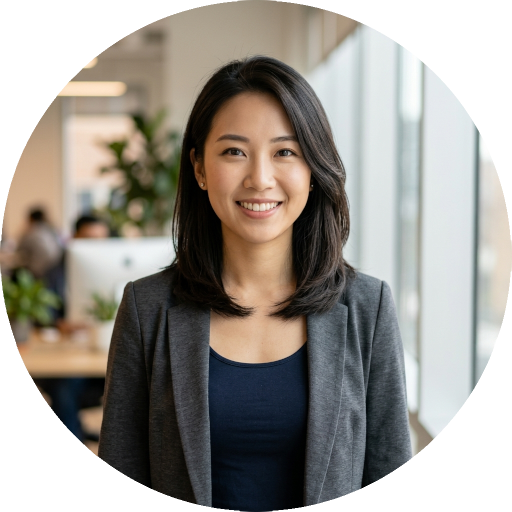
\includegraphics[width=0.47\linewidth]{profile} 
		\end{center}
        
        \vspace{10pt}
        {\color{ColorAccent}\rule{50mm}{1pt}}\par
        
        \sideSection{Contact}
        {\color{sidebartxt}\fontsize{8.5}{14}\selectfont
          \faPhone{}\enspace +1 (206) 555-0187\par
          \faEnvelope{}\enspace victoria.chen@email.com\par
          \MVAt\enspace \href{https://victoriachen.dev}{\color{ColorAccent}victoriachen.dev}\par
          \faLinkedin{}\enspace \href{https://linkedin.com/in/vchen}{\color{ColorAccent}/vchen}\par
          \faGithub{}\enspace \href{https://github.com/vchen-dev}{\color{ColorAccent}/vchen-dev}\par
          $\triangleright$\enspace Seattle, WA, USA\par
        }
        \vspace{10pt}
        {\color{ColorAccent}\rule{50mm}{1pt}}\par
		
		\vspace{10pt}
        
		\sideSection{Tech Stack}
        \skillbar{JavaScript / React / TypeScript}{0.90}
        \skillbar{Node.js / Express / Backend}{0.88}
        \skillbar{SQL (PostgreSQL / MySQL)}{0.92}
        \skillbar{System Design \& Architecture}{0.85}

		\vspace{5pt}

        \sideSection{Tools \& Stack}
        {\fontsize{7}{11}\selectfont\linespread{1.2}\selectfont\raggedright
          \tagG{React} \tagG{Node.js} \tagG{AWS} \tagG{Docker}\\[3pt]
          \tagG{PostgreSQL} \tagG{MongoDB} \tagG{Git/GitHub} \tagG{REST APIs}\\[3pt]
          \tagG{Webpack} \tagG{Jest/Testing} \tagG{CI/CD}\par 
        }

		\vspace{15pt}

        \sideSection{Languages}
        {\color{sidebartxt}\fontsize{8.5}{13}\selectfont
          English --- Native\par
          Spanish --- Intermediate\par
        }
        
   		\vspace{10pt}
   		
        \sideSection{Certifications}
        {\color{sidebartxt}\fontsize{8}{11}\selectfont
          {\color{ColorAccent}\ding{51}}\enspace AWS Solutions Architect\par
          {\color{ColorAccent}\ding{51}}\enspace Google Cloud Associate\par
          {\color{ColorAccent}\ding{51}}\enspace React Advanced Developer\par
          {\color{ColorAccent}\ding{51}}\enspace MongoDB Database Expert\par
        }
    };
  \end{tikzpicture}
}


%%%%%%%%%%%%%%%%%%%%%%%%%%%%%%%%%%%%%%%%%%%%%%%%%%%%%%%%%%%%

\vspace*{.5em}
\mainSection{Professional Profile}
{\fontsize{9}{13}\selectfont\color{ColorMainText}


Full-stack software engineer with 6+ years of hands-on experience building scalable web applications using \textbf{JavaScript/TypeScript} and \textbf{Node.js}. Specialized in modern React architectures for responsive, user-centric frontend experiences and server-side development with Express.js and cloud-based solutions.

Proficient in designing and implementing microservices, RESTful APIs, and database solutions leveraging PostgreSQL and NoSQL technologies. Experienced with cloud infrastructure on AWS, containerization with Docker, and CI/CD automation to ensure reliable deployments.

My approach emphasizes clean code principles, comprehensive testing strategies using Jest and integration tests, and collaborative development practices following agile methodologies.

}\par

\mainSection{Featured Projects}

\project%
  {EcoTrack --- Sustainability Platform}%
  {Personal Project / 2024--2025}%
  {\tagB{React}\tagB{Node.js}\tagB{PostgreSQL}}%
  {%
    \item Full-stack web application for tracking carbon footprint and environmental impact. Built with React frontend and Node.js/Express backend with real-time data visualization.
    \item Implemented responsive UI with Tailwind CSS, JWT authentication, and integrated third-party APIs for carbon calculation algorithms.
  }%
  {github.com/example/ecotrack}
  
\project%
  {TaskFlow --- Collaborative Project Management Tool}%
  {Tech Innovation Labs / 2023 -- 2024}%
  {\tagB{React}\tagB{TypeScript}\tagB{MongoDB}}%
  {%
    \item Developed full-featured project management SaaS application with real-time collaboration capabilities using WebSockets.
    \item Designed scalable backend API with MongoDB, implemented complex filtering and search functionality, and created intuitive team dashboard components.
  }%
  {github.com/example/taskflow}

\project%
  {DataViz Dashboard --- Analytics Frontend Framework}%
  {Open Source Contribution / 2023}%
  {\tagB{React}\tagB{D3.js}\tagB{TypeScript}}%
  {%
    \item Created reusable React component library for interactive data visualization with 20+ chart types and real-time data binding.
    \item Optimized rendering performance for large datasets and published as npm package with comprehensive documentation and examples.
  }%
  {github.com/example/dataviz-dashboard}

\mainSection{Work Experience}
{\fontsize{10}{12}\selectfont\bfseries\color{ColorMainText}
  Senior Full-Stack Software Engineer}\par
{\fontsize{8.5}{11}\selectfont\color{ColorMuted}
  Cloudwave Technologies Inc. / 2020--Present}\par
\vspace{4pt}
{\fontsize{9.5}{13}\selectfont\color{ColorMainText}
  \begin{itemize}
    \item Led development of customer-facing web platform serving 500K+ monthly active users, architecting frontend with React and backend services with Node.js.
    \item Established best practices for code quality, testing standards, and CI/CD pipelines that reduced deployment time by 60\%.
  \end{itemize}
}

\mainSection{Academic Background}
{\fontsize{9.5}{14}\selectfont\color{ColorMainText}
  \textbf{Bachelor of Science in Computer Science} \hfill \textcolor{ColorMuted}{2019}\\
  \hspace*{1em}University of Washington, Seattle\par\vspace{4pt}
}

\medskip

\mainSubsection{Cloud, Frontend and Modern Web Technologies}
\cert{2024}{AWS Solutions Architect Associate Certification}{Amazon Web Services}
\cert{2024}{Advanced React and Performance Optimization}{Udemy / React Academy}
\cert{2023}{Node.js and Express.js Mastery}{Coursera / IBM}
\cert{2023}{Google Cloud Associate Cloud Engineer}{Google Cloud}
\cert{2022}{TypeScript Advanced Programming Concepts}{Frontend Masters}

\mainSubsection{Database Design and API Development}
\cert{2024}{PostgreSQL Advanced: Performance Tuning}{Pluralsight}
\cert{2024}{MongoDB Advanced: Indexes and Aggregations}{MongoDB University}
\cert{2023}{RESTful API Design and Best Practices}{Udemy}
\cert{2023}{GraphQL Fundamentals and Apollo Client}{Apollo University}
\cert{2022}{API Security and Authentication Standards}{OWASP / Coursera}

\mainSubsection{Professional Development and Leadership}
\cert{2023}{Agile Project Management for Development Teams}{PMI}{}{}{}
\cert{2022}{Technical Leadership and Mentoring}{O'Reilly Media}

\mainSubsection{Advanced Professional Training}
\cert{2019}{Full Stack Web Development Bootcamp Certification}{General Assembly}
\cert{2020}{Advanced JavaScript: ES6+ and Functional Programming}{Egghead.io}
\cert{2021}{Web Application Security Best Practices}{SANS Cyber Aces}


\end{document}
